\documentclass[11pt]{elegantbook}
\title{Lesson Plan Journal}

\subtitle{Mrs. Patricia Toelle's 8th-Grade Math Classes \\ at Perry
  Heights Middle School}

\author{Randall Helzerman}
\institute{University of Evansville}
\date{\today}
\version{0.1}

%\bioinfo{Bio}{Information}

\cover{cover.png}
\usepackage{tikz}
\usepackage{array}
\renewcommand{\arraystretch}{2}

% modify the color in the middle of titlepage
\definecolor{customcolor}{RGB}{32,178,170}
\colorlet{coverlinecolor}{customcolor}
\usepackage{cprotect}

\usepackage{colortbl}
\usepackage{xcolor}
\usepackage{graphicx}
\usepackage{blindtext}

\usepackage{tabularx}
\newcolumntype{Y}{>{\centering\arraybackslash}X}

\usepackage{pdfpages}

\addbibresource[location=local]{reference.bib} % bib

\begin{document}

\maketitle

\frontmatter
\tableofcontents

\mainmatter

%\preface

\part{August}

\chapter{8/4/2025 through 8/9/2025}

This is a reflection on the first week of classes, being a Student
Teacher in Mrs. Patricia Toelle's 8th grade Math classes.  I am
rolling up the entire first week into a single reflection, because
what happened in the first 5 days divides more naturally into thematic
categories, not temporal categories.

\section*{The room and use of physical space}

Perry Heights Middle School is a very charming school, with a small
(440ish) number of students, and a correspondingly small physical
plant, and, alas, correspondingly small rooms.
ways--fitting all the necessary desks takes up almost all of the free

However, I think that perhaps these smaller rooms might feel more cozy
and reassuring to a middle school student, compared with the vast
cavernous rooms which Central High School had.  The rooms and hallways
are carpeted, which was a big surprise to me, as I've never been in a
school which didn't use industrial-grade linoleum.  However, it does
make the room somehow softer and warmer.  In addition, my aging ankles
appreciated standing on a softer surface all day!

\section*{Use of wall space}

The lion's share of the wall space is taken up by 4 whiteboards, which
are used for stations for activities.  One of the whiteboards has four
pencils stuck on, and next to them a space for a child to write their
name when they borrow a pencil. This is an excellent system, IMHO.

Nestled between is a series of posters which I hope will change the
lives of both the students and myself: posters which show various
slogans illustrating the growth mind set.  Thoughts become words, words
become actions, actions become habits.

\section*{Activities and Rituals}

To further show the growth mind set, Mrs. Toelle gave the children a
baggy of statements like ``I tried it and it didn't work'', and ``I'll
find another way to do it'', things like that.   She had the children
sort the statements as to whether they were characteristic of the growth
mind set or the fixed mind set.

Interestingly, the children were able to sort the statements quite
accurately.  Now that they know the growth mind set, lets hope they
practice it!

Side note: I'm trying to adopt a growth mind set myself w.r.t. parts of
teaching which have been hard for me, such as learning the student's
names.  There are about 75 students in our classes, and I've learned
about 60 names....not reaching the goal of learning them all by the
end of the first week, but frankly more names than I learned at either
Bosse or Central.

Mrs. Toelle has a ritual called the ``community circle'' which I think
was used very effectively.  The kids all gather in a circle, and she
asks a question designed to let us get to know more about ourselves.
Examples include ``what was the funniest thing you did this summer''
and ``what are you most dreading about the semester.''

She then gives students a few minutes to think.  When a student has an
answer, they give a thumbs up.  When a quorum of thumbs are up we pass
a ``magic marble'' around the circle, and the one holding the marble
is the only one allowed to speak.  I say a quorum and not every
student, because the student always has the right to just say
``pass.''  They do, however, have to say their name, which I appreciate
very much, as it aids in learning their names quite considerably.

I am not a superstitious man, but I am almost prepared to believe it
is a magic marble, because all Mrs. Toelle has to say is ``Respect the
Marble!!'' and all side chitter-chatter stops.   Astounding.

\section*{On the teaching of 8th graders}

I had some trepadations about whether I would be compatible with 8th
graders.  I never taught a freshman class, but I did hear other
teachers complaining about how ill-behaved the freshmen were.

While it is true, these children are not as mature as the juniors and
seniors I have taught before, they are unambiguously {\em children},
which means that sure they have more exuberance than upperclassmen do,
they also are more responsive to adult guidance.   

I'm delighted to announce that I absolutely love working with 8th graders.
I was not at all uncomfortable joining in the activities, yelling out
the slogans, etc.  These children have fortunately not had all of the joy
of life beaten out of them yet.  Even playing a game like ``four corners'',
just scurrying across the room--merely walking on the floor--was a
source of delight for them.

I certainly hope that I can help them mature intellectually and
morally, without squashing that thrill they have of just being alive.

\chapter{Monday, 8/11/2025}

\section*{Community Circle}

An interesting thing happened when we did the community circle with
the flowing question: ``What I need to feel safe in class''.  A few of
the students were brave enough to give answers like ``I need the
teacher to not make me feel stupid if I answer a question wrong.''
But most were very uncomfortable answering this question in the
standard community circle format.  Most of the students passed.

So Mrs. Toelle came up with an alternate plan: have the children write
down what they needed to feel safe anonymously, on sticky notes.
It was important that this was anonymous, as evinced by a student
who didn't hear at first that they were to be anonymous, but found out
halfway through his note.  He said, ``We don't write down our names?
That changes everything!''  Then he proceeded to erase what he set down
and write out what he really needed.

\section*{IXL}

The students are required to finish 20 minutes of IXL a week, which is
a computer-based series of questions, individualized for each student
based on their current mastery.  They are required to get an 80%
score.

Mrs. Toelle uses this as a way for students to demonstrate that they have
put in effort to learn the material as a pre-requisite for re-taking tests.

\section*{Workbook Assignment}

The students are then given the opportunity to work thorough exercises
in their workbook, in order to learn how to write very large numbers
and very small numbers in terms of powers of 10.  The workbook has a
handy graphic organizer which lets the students figure out whether, 
say, 0.009 has its first nonzero digit in the tenths, hundrethds, or
thousandths place.



\chapter{Tuesday, 8/12/2025}

\section*{Intro, warm up}

Mrs. Toelle had a few what she called ``fluency'' exercises, meant to
bridge from what the students hopefully remembered to what they needed
to learn today.

The first few problems displayed on the Promethean board were examples
of writing large numbers like 8,000,000 as a digit times 10 to some
power.

She then had them try to estimate the following two quantities:
\begin{enumerate}
\item How many different subway sandwiches can be made by combining
  ingredients?
\item How large is a single COVID virus?
\end{enumerate}

\noindent I noted with interest that the student's estimations were
off by at least two orders of magnitude in either direction.  But the
point wasn't to get the right answer, the point was whether you could
express your guess as a number.

\section*{Main subject matter}

The main lesson consisted of exercises and practice in converting
large numbers to and from exponential notation.  ``Exponential
notation'' is a variant of scientific notation, which, curiously, does
not use negative exponents (e.g. $10^{-1}$ for numbers less than 1.
Instead, they used reciprocals of powers of 10. (i.e. $\frac{1}{10^{2}}$.

Frankly, I have mixed feelings about this, as it is non-standard
notation.  But, it is not {\em incorrect} notation, and they are
careful not to call it ``scientific notation'' but rather
``exponential notation.'' And I cannot deny that it is a smoother
on-ramp.

\section*{Landing, evaluation}

One session (session 3/4) was on schedule enough to be able to take
what is termed an ``exit ticket.''  It is printed on a sheet in their
workbooks, which they are obliged to rip out and complete.

It consisted of about 4 problems which are meant to be very easy if
the student has understood the lessons.  How were these used? Stay
tuned for tomorrow's reflection.


\chapter{Wednesday, 8/13/2025}

\section*{Small Groups to review exit ticket}

The exit tickets from yesterday have already been graded, and the
children are who did not get $100\%$ have been categorized into small
groups for a more focused instruction.  The groups are divided up
between Mrs. Toelle and myself.  We then re-explain the concept, have
them drill on a few problems, and then correct their exit ticket.

\section*{IXL practice}

For the students who did get $100\%$, and for the students who have
corrected their exit tickets, we have them practicing on their IXL
problems.

\section*{Fluency and In-class practice}

After the the small groups, we do another fluency exercise for review,
followed by in-class practice from the workbook.

\section*{Exit ticket for classes 1/2 and 8/9}

Classes 1/2 and 8/9 had a chance to take the exit ticket which class
3/4 took the day before,



\chapter{Thursday, 8/14/2025}

\section*{Small Groups}

The exit tickets for classes 1/2 and 8/9 had been graded, so the children
were assigned to smaller groups as was done for class 3/4 the day before, and
given more focused tutelage in smaller groups, while the rest of the class
did their IXL assignments.

\section*{Fluency and independent practice}

Afterwards, the class did the fluency exercise, and then was given
time for in-class practice in their workbooks.  Afterwards, the
answers were checked.


\chapter{Friday 8/15/2025}


\section*{Observation of Honors Geometry Class}

Mrs. Toelle did me a solid and arranged for me to observe Mrs. Rice's
honors geometry class.  I had heard rumors of a mythically good
teacher, but what I saw with my own eyes utterly exceeded any report,
and indeed, and expectation that I could have had.

\section*{Description of classroom, and how it serves the learning process}

The classroom was bigger than the usual cozy Perry Heights classroom.
In contradistinction to what one would imagine that an 8th-grade
classroom was like (every square inch of the walls decorated with cosy
pictures or encouraging slogans) the decor was spare, even stark.
Apparently, the honors students are already in possession of a growth
mindset, and do not need to be reminded of slogans to maintain it.

The desks were arranged in islands of 6 to 8 desks put together such
that the children all faced each other, and yet could all also turn to
see the Promethean board at the front of the class.

This was for to provide an opportunity for groups of students to work
and struggle together.  Mrs. Rice strongly believes that it is
important for student to struggle together like this. This is in
contradistinction with most of my previous mentors who strongly
objected to any teaching technique which would cause the students to
feel perplexed for any length of time.

\section*{Teaching}

Interestingly, the students were not issued a workbook, or even a textbook.
Instead, they were issued graph-lined notebooks, like the notebooks
I used to use as a professional engineer.  The students were expected
to take notes in the notebook with a high enough fidelity that they
could refer back to it well enough not to need a textbook or workbook.
This is a very useful skill, which I used on the job every day.

The class opened with a tutorial of how to use a compass--compasses
having been previously passed out.  Now, I cannot resist commenting on
what passes for compasses these days.  As a card-carrying member of Gen X,
we did not have the safety concerns which are so prevalent today.
For us, a compass was something which could literally (not metaphorically or
hyperbolically, but {\em literally}) be used as a lethal weapon, what with its
long, pointed, and very sharp end.  I.E., what students in every western
nation have been using as compasses since the days of Alexander the Great.

The instrument which was given to the kids had no such sharp pointing
parts.  It was basically a ruler with a pivot on one end which could
be held with a finger, and a sliding member which had a hole you could
put a pencil point into, and then you could pivot it around to draw a
circle.

I have very mixed feelings about this.  The whole game of geometry is
to see how far you can get with just a straight-edge and a compass.
On the one hand, I suppose that it is cool that the functionality of
both instruments can be combined into one, kind of.  On the other
hand, this does put them at a distance them from both the historical
roots of geometry, which is bad enough, but it also obscures the very
different roles which the two instruments play.  The ruler defines
what a straight line is, and the compass defines what it means to say
that two lengths are equal.

Nevertheless, I felt very privileged to be with these students at the
very moment they were learning how to use a compass.  It was a sacred
moment.

\section*{STRUGGLE!!}

Mrs. Rice proceeded to give them an assignment: use this compass to
bisect a line segment.  This is something which is easy to do once you
see the trick, but it is actually rather hard to come up with the
trick.

So she set the groups of students to chew on it, and so they did.
They were a classroom of 8th-graders, so naturally, there was plenty
of gigging and it was obvious the students were enjoying each other's
company.  But they did indeed struggle with the problem.  For a long
time!  Not every group could find the trick, but, when the trick was
revealed, there was a palpable sense of ``ah ha!!!!'' in the
classroom.  I never forgot how to bisect a line with a compass, and
I'm sure that these students--after having struggled for the
knowledge, will never forget either.

\section*{Techniques learned}

After the class, Mrs. Rice was kind enough to answer my questions and
share some new techniques.  One killer technique she showed me--not
for this geometry class, but for an algebra class-- was a poster-sized
graphical organizer she used to get students familiar with the
integers and how they are composed of prime factors.  The poster had
numbered boxes for numbers from 1 to 500.  She had the students put a
red sticker on every other number--those are the even numbers,
divisible by 2.  Then she had them put a green sticker on every third
box--those are the numbers divisible by 3.  Then a yellow sticker for
every 5th box--the numbers divisible by 5.

I thought this was an amazing technique, because it doesn't matter
whether a student is a verbal learner, a visual learner, or a
procedural learner, after doing this exercise, any student would be
able to grasp on a very visceral level the fact that all numbers are
composed of prime factors.  And 8th-graders are still young enough to
love stickers, so I'm sure they had a really fun time doing the
exercise.

What's more,the poster would be useful for them when learning how to,
say, find greatest common factors or least common multiples, factoring
polynomials, etc etc.

\section*{Sad postscript}

I was wondering how Mrs. Rice could possibly get away with teaching
her students like this.  Certainly any time I tried to let my students
struggle, or I strayed off of the EVSC-mandated script, it was a point
of contention with my mentors.

I knew that EVSC has mandated what textbooks, workbooks, and even
lesson plans were to be used, and I mean used line-by-line, letter by
letter.  I suppose this gives a uniformity to instruction across
EVSC. But this drains the teacher of any discretion to use their own
unique talents adapted to their own unique group of students in their
own classroom.

When I asked Mrs. Rice how she could do this, she said, ``Well, I
suppose I could be written up for not following the EVSC lesson plans.
If they fire me I'll just go do something else...''


\chapter{8/18/2025 through 8/22/2025}

The focus of this week was to give the students a very firm grasp of
the rules governing the evaluation of mathematical expressions
containing exponents.

For this week generally, I will be incorporating lesson plans written
according to a standard format.  This is because this was the first
week where some of the teaching content was created by me, and which I
taught during parts of the lecture.  I wish to emphasize however that
the bulk of the lessons are still being prepaired and given by
Mrs. Toelle; Unless otherwise noted, my contributions this week are in
the section entitiled ``Introduction/Anticipatory Set'' but in the
classroom we call the ``Fluency'' exercise.

Figure \ref{qqt_ex} shows a pdf of the ``Quiz-Quiz Trade'' cards which I made.
They can be printed out and cut along the guidelines to fit on 3x5
cards.  Many thanks to Mrs. Toelle for reviewing them for aptness and
correction.

\pagebreak
\begin{figure}[h]
  \begin{minipage}[t]{5in}
    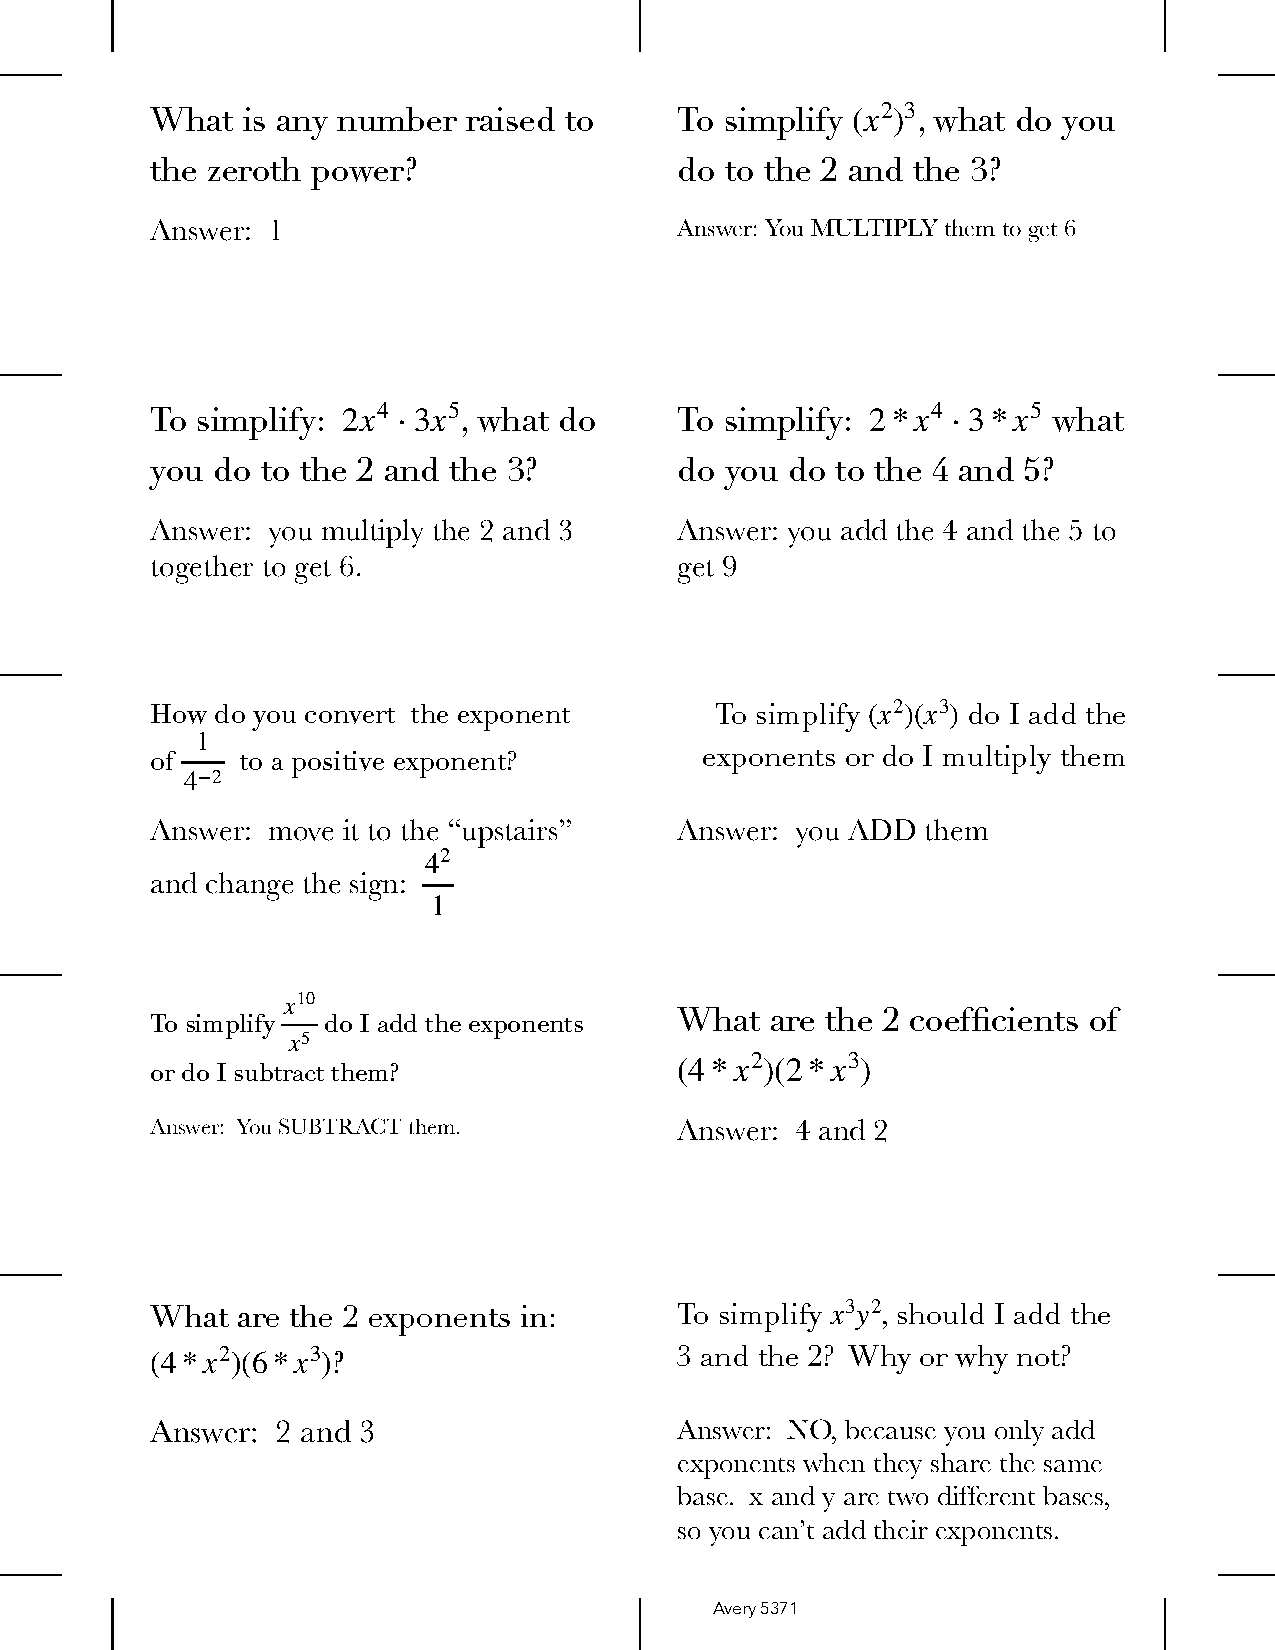
\includepdf[page=1, scale=0.65]{qq_t.pdf}
    \caption{Quiz-Quiz Trade cards for exponents}
  \end{minipage}
  \label{qqt_ex}
\end{figure}
  


\begin{tabularx}{\textwidth}{Y}
  {\large University of Evansville Lesson Plan Format } \\
  \arrayrulecolor{blue} \hline \\
\end{tabularx}


\arrayrulecolor{black} 
\begin{tabularx}{\textwidth}{|X|X|}
  \hline 
  \textcolor{blue}{Name:} Randall Helzerman         &   \textcolor{blue}{Student ID Number:} 0128861 \\
  \hline 
  \textcolor{blue}{Course Number:} EDUC-497-03 2025FA &   \textcolor{blue}{Instructor Name:} Dr. Laura Watkins\\
  \hline 
\end{tabularx}
\arrayrulecolor{black} 

\vskip 10pt

\begin{tabularx}{\textwidth}{Y}
  {\bf Lesson Overview} \\
\end{tabularx}
\arrayrulecolor{black}


\arrayrulecolor{black} 
\begin{tabularx}{\textwidth}{|X|X|}
  \hline 
  \textbf{Lesson Title: Applying Rule of Exponents} \\
  
  \hline 
  \textbf{Subject:} Math\\
  
  \hline 
      {
        \begin{tabularx}{\textwidth}{X|X}
          \hskip -6pt
          \textbf{Duration of Lesson:} 80 min & \textbf{Grade Level(s)/Course:} 8th grade\\
        \end{tabularx}
      } \\
      
      \hline
      
      \textbf{Lesson Description:}  \\
        
        \hline
        
        \textbf{Standards and/or Indicator(s):}  \\
        \textbf{Indiana Standard number:} 8.NS.3 \\
        \textbf{Text:} Given a numeric expression with common rational
        number bases and integer exponents, apply the properties of
        exponents to generate equivalent expressions.  \\
        \hline
        
        \textbf{Learning Objective(s)/Target:} {\tiny What do I want students to learn and be able to do at the end of the lesson? (I can statements)}
               {\begin{enumerate}
                 \item I can identify which rule of exponents is needed to simplify.
               \end{enumerate}} \\
               \hline
               
               \textbf{Lesson Resources/Technology: }  Cards numbered 1 thorugh 14 to mark ``stations'' around the room, and 12 cards with problems involving exponentials.\\
               \hline
               
               \textbf{Key Vocabulary:} {\tiny List all key vocabulary words that will be taught to help students understand the concepts in the lesson.} \\
               \hline
\end{tabularx}
\arrayrulecolor{black}

\pagebreak

\begin{tabularx}{\textwidth}{|p{0.5in}|X|}
  \hline
  \centerline{\textbf{\large Time}} &  \textbf{\large Instructional Sequence } \\
  \hline
  \textbf{10-20min} &  \textbf{\em Introduction/Anticipatory Set:}  Six problems involving eponentials were written on the board.   Then we proceed in 2 stages:
         {\begin{enumerate}
           \item For all 6 problems, students first write down the rule needed to simplify the expression.  We review the answers.
           \item Then the students solve the problems.  We review the answers.
         \end{enumerate}}\\
         \hline
         \textbf{10-20 min} &  \textbf{\em Demonstrate, Build, Apply Knowledge} Mrs. Toellle had the students to to page 81/82 in the workbook, which was where the students should have written down the various rules for \\
  \hline
  \textbf{N/A} &  \textbf{\em Depth of Knowledge Questions:} N/A \\
  \hline
  \textbf{10-20 min} &  \textbf{\em Guided Practice:} Worked through a study guide for the test to be given the next day. \\
  \hline
  \textbf{10-20 min} &  \textbf{\em Independent Practice:} An Edulastic problem set was given. \\
  \hline
  \textbf{1 min} &  \textbf{\em Assessment:} Edulastic lets the students check their answers 1 time, and all the results are wrappted up to give a read on how the students aer doing. \\
  \hline
  \textbf{10-20 min} &  \textbf{\em Wrap Up/Closing Activity/Reflection:} We did a ``math treasure hunt.''   Around the room cards with numbers from 1-14 were posted, which marked stations around the room.  At each station, there was a problem involving exponentials.  Underneith that was printed the answer to the problem at{\em a different} station around the room.   \\
  \hline
\end{tabularx}

\vskip 6pt

\begin{small}
\begin{tabularx}{\linewidth}{|p{2.1in}|X|}
  \hline
  \textbf{Differentiation/Accommodations and/or Modifications: } & \\
  \hline
  \textbf{Culturally Responsive Teaching/ Diversity and Inclusion: } & \\
  \hline
\end{tabularx}

\vskip 6pt

\begin{tabularx}{\linewidth}{|X|}
  \hline
  \textbf{Self-Reflection:} \\
  \textbf{My Teaching:} 
  \begin{enumerate}
  \item The big idea from the previous day as a metaphor, viz, that the problems were locks, and the rule of exponents were the keys to solve them.  In retrospect, this would have been more effective if the 
  \item .
  \end{enumerate} \\
  
  \textbf{The Students:}
  \begin{enumerate}
  \item .
  \item .
  \end{enumerate} \\
  
  \textbf{The Lesson:}
  \begin{enumerate}
  \item .
  \item .
  \end{enumerate} \\
  
  \hline
\end{tabularx}
\end{small}


\begin{tabularx}{\textwidth}{Y}
  {\large University of Evansville Lesson Plan Format } \\
  \arrayrulecolor{blue} \hline \\
\end{tabularx}


\arrayrulecolor{black} 
\begin{tabularx}{\textwidth}{|X|X|}
  \hline 
  \textcolor{blue}{Name:} Randall Helzerman         &   \textcolor{blue}{Student ID Number:} 0128861 \\
  \hline 
  \textcolor{blue}{Course Number:} EDUC-497-03 2025FA &   \textcolor{blue}{Instructor Name:} Dr. Laura Watkins\\
  \hline 
\end{tabularx}
\arrayrulecolor{black} 

\vskip 10pt
  
\begin{tabularx}{\textwidth}{Y}
  {\bf Lesson Overview} \\
\end{tabularx}
\arrayrulecolor{black}


\arrayrulecolor{black} 
\begin{tabularx}{\textwidth}{|X|X|}
  \hline 
  \textbf{Lesson Title:} Final Prep for Test on Exponentials \\
  
  \hline 
  \textbf{Subject:} Math\\
  
  \hline 
      {
        \begin{tabularx}{\textwidth}{X|X}
          \hskip -6pt
          \textbf{Duration of Lesson:} 80 minutes & \textbf{Grade Level(s)/Course:} 8th grade\\
        \end{tabularx}
      } \\
      
      \hline
      
      \textbf{Lesson Description:} Final Prep for Test on Exponentials  \\
        
        \hline
        
        \textbf{Standards and/or Indicator(s):} \\
        \textbf{Indiana Standard number:} 8.NS.3 \\
        \textbf{Text:} Given a numeric expression with common rational
        number bases and integer exponents, apply the properties of
        exponents to generate equivalent expressions.  \\
        \hline
        
        \textbf{Learning Objective(s)/Target:}
             {\begin{enumerate}
               \item I can multiply terms containing exponents.
               \item I can identify coefficients in a term.
               \item I can identify bases in a term.
               \item I can identify exponents in a term.
               \item I can look at a term and see which rule of
                 exponents can be used to simplify it.
               \item I can solve simple equations using exponents.
             \end{enumerate}} \\
               \hline
               
               \textbf{Lesson Resources/Technology: }  3x5 index cards (30 count), with questions about exponentials printed out and taped to the front side, and corresponding answers printed out and taped to the back side.  \\
               \hline
               
               \textbf{Key Vocabulary:} Coefficient, Exponent, Base  \\
               \hline
\end{tabularx}
\arrayrulecolor{black}

\pagebreak

\begin{tabularx}{\textwidth}{|p{0.5in}|X|}
  \hline
  \centerline{\textbf{\large Time}} &  \textbf{\large Instructional Sequence } \\
  \hline

  \textbf{10 min} & \textbf{\em Introduction/Anticipatory Set:} 6
  terms are written on the board, and students are to simplify the
  expressions using the rules of exponents.  The students use their
  whiteboards to write their answers, and when they are finished, they
  stand up.
  
  When about 80 percent of the class has stood up, have them sit down
  and discuss the answers they got with their partner for a few
  minutes.

  Then review the answers with the class. \\
  \hline
  
  \textbf{N/A} &  \textbf{\em Demonstrate, Build, Apply Knowledge} \\
  \hline
  \textbf{10 min} &  \textbf{\em Depth of Knowledge Questions:} Previously assigned workbook questions are reviewed.  \\
  \\
  \hline
  \textbf{N/A} &  \textbf{\em Guided Practice:} N/A \\
  \hline
  \textbf{10 min} &  \textbf{\em Independent Practice:} A game called ``Quiz-Quiz Trade'' was played.  A 3x5 card is given to every student.  On one side, there is a question about the rules of exponents.  On the other side is the answer.  The game proceeds by repeating the following steps:
 
  {\begin{enumerate}
    \item Students stand up and go around the classroom, looking for somebody who they haven't quizzed yet.
   \item (The ``Quiz-Quiz'' step) The students take turns asking their
     partner the question on the card they have.  The partner gives and answer, and which is checked against the correct answer on the back of the card.
   \item (The ``Trade'' step)  Then the students exchange cards, and go find somebody they haven't done this yet with.
 \end{enumerate}} \\
 \hline
 
 \textbf{40 min} &  \textbf{\em Assessment:}  The first test of the semester was administered to them. \\
 \\
 \hline
 \textbf{N/A} &  \textbf{\em Wrap Up/Closing Activity/Reflection:} After finishing the test, the students were encouraged to take a little quiz which determines whether they are language, visual, or kinesthetic learner. \\
 \hline
\end{tabularx}

\vskip 6pt

\begin{small}
  \begin{tabularx}{\linewidth}{|p{2.1in}|X|}
    \hline
    \textbf{Differentiation/Accommodations and/or Modifications: } & One of our sessions is an inclusion class, and students who were not comfortable socially were allowed to opt out, while an Aide reviewed with them.\\
    \hline
    \textbf{Culturally Responsive Teaching/ Diversity and Inclusion: } & N/A \\
    \hline
  \end{tabularx}
  
\vskip 6pt

\begin{tabularx}{\linewidth}{|X|}
  \hline
  \textbf{Self-Reflection:} \\
  \textbf{My Teaching:} 
  {\begin{enumerate}
  \item I am wondering whether the ``Quiz-Quiz Trade'' questions were extensive enough to prep them for the test.
  \item it is a delicate balancing act: one one hand, we want enough questions to cover what needs to be reviewed.  On the other, we want as few questions as possible, so the students see them over and over again, giving them a robust review of the material.
  \end{enumerate}} \\
  
  \textbf{The Students:}
  {\begin{enumerate}
  \item 8th graders are so fun.  They loved the ``Quiz-Quiz Trade''
    game.  They enthusiastically played it with each other, and kept
    trading partners until we ran out of time. I don't think my
    upperclass math classes which I have taught would have reacted as
    enthusiastically.
  \end{enumerate} }\\
  
  \textbf{The Lesson:}
  {\begin{enumerate}

    \item The ``Quiz-Quiz Trade'' game is remarkably effective at
      getting kids to actually attempt to answer the questions and
      review the material.
      
    \item If we had just put the same questions on a worksheet, for
      example, 80 percent of the class would have started working on
      them, reluctantly, 10 percent would have worked on them after
      direct teacher interaction, and 2 or 3 would have not worked on
      them at all.  Yet they all went around asking each other
      questions and giving answers.  Astounding.

    \item We just set a timer to let us now when to stop playing the
      game, but perhaps we should introduce some more formal mechanism
      to track whether each kid is getting a chance to talk with every
      other kids.  Mrs. Toelle assures me that 8th-graders still love
      stickers, so perhaps we should give a sheet of stickers to every
      student, and then have them past them on a sheet, and when
      they've collected all of the stickers they know they are done.

    \item I'm wondering whether we should do a round of ``Quiz-Quiz
      Trade'' every day, or perhaps several times per day, after 10
      minutes of lecture telling them how to do the problems on the
      cards.  It gets kids up out of their seats, walking and
      oxygenated and therefore fully awake, and--importantly--doesn't
      let any student just opt-out of class by zoning out during the
      lectures and then refusing to do the workbook problems.

  \end{enumerate} }\\
  \hline
\end{tabularx}
\end{small}



\chapter{8/25/2025 through 8/29/2025}

Notable events this week: (will be expanded upon in lesson plans:)

\begin{itemize}
  
\item Giving one entire class on Tuesday.
  
\item Giving all of the classes on Thursday and Friday.
  
\item I designed the fluency and theactivities, but the ret of the
  lesson plan was designed by Mrs. Toelle, even when given by me.
  
\item Identified a vocablary deficiency in some students which was
  impeding learning, and fixed it with pulling a smaller group.
  
\end{itemize}

\section{Spotlight on Student ``D''}

I'll call him ``D'' for privacy reasons.  D is African American,
handsome, wears his hear long and pulled into a pony tail.  He is
charismatic, always cheerful, and is liked by everyone.  In addition,
he has about as much energy as a nuclear powerplant.  He reminds me
very much of some salesmen I've known in my previous careers.  Very
sucessful salesmen: those people who you just can't help liking and
have enough energy to make it through endless days and hours of
negotiations in order to close the sale, without ever losing their
good spirits or smiles.

D is small, even for an 8th grader.  He hasn't had his growth spurt
yet, and just as he is physically less mature than the bulk of the
class, he is also emotionally less mature.  He has a hard time staying
in his seat, and faces endless temptations to talk in class-both
because he loves talking, and everybody else loves talking to him.

Alas, these are not the only challenges D faces.  He has been shuttled
back and forth between his mother and grandmother.  He has apparently
also had to live in a homeless shelter for some time. 

When I think about the amount troubles and trials which have been
dumped on D, through no fault of his own, when his is a {\em child},
just 13, and a very youngish 13 at that, it is doubly amazing.  First,
how could we let this happen, and second, how well he's doing.  He is
energetic and talkative, but never disrespectful or rude.  He hasn't
withdrawn from his world, but he is fully engaged.  Whenever there is
some task to be done, like collecting papers or running something to
the office, he always wants to do it.

Well, its my job to teach him math, but I'm hoping that he can teach
{\em me} something about resilience and how to stay cheerful in a very
hard world.  So what to do?  He was falling behind, not writing down
class notes, or doing class assignments.  What is standing in his way?

The first clue was that in class, during the explanations of how to do
the problems, he would sometimes say, ``I don't understand that
word!'' or ``What does that word mean?''.  The clincher was when I
looked at one of his exit tickets, and it was apparent that he
understood the math it was testing, but he got the last question wrong
becaue he misunderstood the question.  It used some vocabuary which he
was just unfamiliar with.

The problem was vocabulary.  When he heard a word he didn't
understand, he stopped taking notes becase he was confused. I raised
the issue in our PLC, and Mrs. Toelle suggested I pull him and another
student for seperate instruction.  The lesson was about how to use
Desmos to find square roots and cube roots.  He very quickly learned
how to use Desmos to find square roots.  He actualy is pretty good at
math!  But he had a problem doing cube roots....what gives?

Yeah, apparently Desmos has {\em two} different calculators, one which
has a button for cube roots and one which only has a square root
button.  Even I didn't know how to pull up the right one, thank
goodness the other student I pulled knew how.  The next day, when he
rejoined the class, thank-goodness Mrs. Mosby noticed he was still
using the wrong calculator!

When I was reviewing how to do cube roots with the class, D put his
hand up and said ``I know I know!!  Can I come up and show everybody
how to do it?''  So I pulled up the desmos calculator on the
promethean board, and sure enough D came up and--after hunting for the
right calculator--found the right button and found the cube root of
125 in front of the entire class!

It was a trick I learned during my other internships...some students
want to be the center of attention, but you can channel that desire
into a very strong motivation to learn math, if you let them be the
center of attention when solving a math problem :-)

The next day, We followed up with a Quiz-Quiz Trade activity
which featured questions about the vocablary used to pose and solve
square and cube and root problems. (See figure \ref{qqt_root})

I'm only going to have 4 more months with D.  I hope he doesn't end up
like countless of my Juniors and Seniors did when I was teaching
Algebra II....we lost them somewhere in middle school math, and they
never really were able to get back on board.  We didn't lose D today,
but all the other challenges he faces have not gone away, and a lot
can happen between now and when he takes Algebra II.

\section{Lesson Plans}

\include{lp_aug_25}

\begin{tabularx}{\textwidth}{Y}
  {\large University of Evansville Lesson Plan Format (8/} \\
  \arrayrulecolor{blue} \hline \\
\end{tabularx}


\arrayrulecolor{black} 
\begin{tabularx}{\textwidth}{|X|X|}
  \hline 
  \textcolor{blue}{Name:} Randall Helzerman           &   \textcolor{blue}{Student ID Number:} 0128861 \\
  \hline 
  \textcolor{blue}{Course Number:} EDUC-497-03 2025FA &   \textcolor{blue}{Instructor Name:} Dr. Laura Watkins\\
  \hline 
\end{tabularx}
\arrayrulecolor{black} 

\vskip 10pt

\begin{tabularx}{\textwidth}{Y}
  {\bf Lesson Overview} \\
\end{tabularx}
\arrayrulecolor{black}


\arrayrulecolor{black}
\begin{tabularx}{\textwidth}{|X|X|}
  \hline 
  \textbf{Lesson Title:} Squares and Cubes and Repeating and Non-repeating
  Decimals\\
  
  \hline 
  \textbf{Subject:} Math\\
  
  \hline 
      {
        \begin{tabularx}{\textwidth}{X|X}
          \hskip -6pt
          \textbf{Duration of Lesson:} 80 min & \textbf{Grade Level(s)/Course:} 8th grade\\
        \end{tabularx}
      } \\
      
      \hline
      
      \textbf{Lesson Description:} In this lesson we get the students
      familier with squares and cubes of small and medium-sized
      integers.  \\
      
      \hline
      
      \textbf{Standards and/or Indicator(s):} \\
      \textbf{Indiana Standard number:} 8.NS.3 \\
      \textbf{Text:} Given a numeric expression with common rational
      number bases and integer exponents, apply the properties of
      exponents to generate equivalent expressions.  \\
      \hline
      
      \textbf{Indiana Standard number:} 8.NS.4 \\
      
      \textbf{Text:} Use square root symbols to represent solutions to
      equations of the form $x^2 = p$, where $p$ is a positive
      rational number. \\
      
      \hline
      
      \textbf{Learning Objective(s)/Target:} {\tiny What do I want
        students to learn and be able to do at the end of the lesson?
        (I can statements)}
      
      {\begin{enumerate}
        \item I can tell when a fraction has a repeating or
          non-repeating decimal.
        \item I can tell when a number is a squared number.
        \item I can tell when a number is a cubed number.
      \end{enumerate}} \\
      \hline
      
      \textbf{Lesson Resources/Technology: } {\tiny (What
        technology will I use? What technology will students
        use for this lesson? What resources will you and/or the
        students need for the lesson – books, mentor texts,
        etc.)} \\ \hline
      
      \textbf{Key Vocabulary:} {\tiny List all key vocabulary
        words that will be taught to help students understand
        the concepts in the lesson.} \\ \hline
\end{tabularx}
\arrayrulecolor{black}

\pagebreak

\begin{tabularx}{\textwidth}{|p{0.5in}|X|}
  \hline
  \centerline{\textbf{\large Time}} &  \textbf{\large Instructional Sequence } \\
  \hline
  \textbf{} &  \textbf{\em Introduction/Anticipatory Set:} {\tiny What meaningful activity will engate students, activate prior knowledge, and prepare students for learning objectives} \\
  \hline
  \textbf{} &  \textbf{\em Demonstrate, Build, Apply Knowledge} {\tiny What meaningful activity will engate students, activate prior knowledge, and prepare students for learning objectives} \\
  \hline
  \textbf{} &  \textbf{\em Depth of Knowledge Questions:} {\tiny Essential questions to extend higher level thinking)
} \\
  \hline
  \textbf{} &  \textbf{\em Guided Practice:} {\tiny (Check for understanding prior to independent work; “We do”)} \\
  \hline
  \textbf{} &  \textbf{\em Independent Practice:} {\tiny (Individual practice, learning centers, reading, composing writing; “You do”)} \\
  \hline
  \textbf{} &  \textbf{\em Assessment:} {\tiny (Evaluate level of student understanding. How will I know if students have achieved today’s learning target?)} \\
  \hline
  \textbf{} &  \textbf{\em Wrap Up/Closing Activity/Reflection:} {\tiny (How will I reinforce/revisit the learning objective? Opportunity for formative assessment. Students reflect on evidence of learning – writing, reading, math target. How will we build on this learning?)} \\
  \hline
\end{tabularx}

\vskip 6pt

\begin{small}
\begin{tabularx}{\linewidth}{|p{2.1in}|X|}
  \hline
  \textbf{Differentiation/Accommodations and/or Modifications: } & \\
  \hline
  \textbf{Culturally Responsive Teaching/ Diversity and Inclusion: } & \\
  \hline
\end{tabularx}

\vskip 6pt

\begin{tabularx}{\linewidth}{|X|}
  \hline
  \textbf{Self-Reflection:} \\
  \textbf{My Teaching:} 
  \begin{enumerate}
  \item .
  \item .
  \end{enumerate} \\
  
  \textbf{The Students:}
  \begin{enumerate}
  \item .
  \item .
  \end{enumerate} \\
  
  \textbf{The Lesson:}
  \begin{enumerate}
  \item .
  \item .
  \end{enumerate} \\
  
  \hline
\end{tabularx}
\end{small}


\begin{tabularx}{\textwidth}{Y}
  {\large University of Evansville Lesson Plan Format } \\
  \arrayrulecolor{blue} \hline \\
\end{tabularx}


\arrayrulecolor{black} 
\begin{tabularx}{\textwidth}{|X|X|}
  \hline 
  \textcolor{blue}{Name:} Randall Helzerman         &   \textcolor{blue}{Student ID Number:} 0128861 \\
  \hline 
  \textcolor{blue}{Course Number:} EDUC-497-03 2025FA &   \textcolor{blue}{Instructor Name:} Dr. Laura Watkins\\
  \hline 
\end{tabularx}
\arrayrulecolor{black} 

\vskip 10pt
  
\begin{tabularx}{\textwidth}{Y}
  {\bf Lesson Overview} \\
\end{tabularx}
\arrayrulecolor{black}


\arrayrulecolor{black} 
\begin{tabularx}{\textwidth}{|X|X|}
  \hline 
  \textbf{Lesson Title:} \\
  
  \hline 
  \textbf{Subject:} Math\\
  
  \hline 
      {
        \begin{tabularx}{\textwidth}{X|X}
          \hskip -6pt
          \textbf{Duration of Lesson:} & \textbf{Grade Level(s)/Course:} 8th grade\\
        \end{tabularx}
      } \\
      
      \hline
      
      \textbf{Lesson Description: {\tiny (Describe the primary nature e.g. hands-on, direct instruction, inquiry, project based etc. of the lesson)}} \\
        
        \hline
        
        \textbf{Standards and/or Indicator(s):} {\tiny Cut and paste from IDOE website here. Feel free to replicate the descriptors listed below to include more standards in this section.} \\
        \textbf{Indiana Standard number:} \\
        \textbf{Text:} \\
        \hline
        
        \textbf{Learning Objective(s)/Target:} {\tiny What do I want students to learn and be able to do at the end of the lesson? (I can statements)}
               {\begin{enumerate}
                 \item I can multiply two positive numbers, a positive
                   and a negative number, and two negative numbers.
                 \item I can tell how many solutions a square root problem has.
                 \item I can tell how many solutions a cube root problem has.
               \end{enumerate}} \\
               \hline
               
               \textbf{Lesson Resources/Technology: } Each desk has a small whiteboard and a marker which the kids can work problems out on.\\
               \hline
               
               \textbf{Key Vocabulary:}  \\
                      {\begin{enumerate}
                        \item Square of a number
                        \item Cube of a number
                        \item Square root of a number
                        \item Cube root of a number
                        \item Square is the inverse of Square root
                        \item Cube is the inverse of a Qube root
                      \end{enumerate}} \\
                      \hline
\end{tabularx}
\arrayrulecolor{black}

\pagebreak

\begin{tabularx}{\textwidth}{|p{0.5in}|X|}
  \hline
  \centerline{\textbf{\large Time} 10min} &  \textbf{\large Instructional Sequence } \\
  \hline
  \textbf{} &  \textbf{\em Introduction/Anticipatory Set:} Put 6 problems on the promethean board.  These are simple mutiplication problems multiplying various combinations of positive and negative numbers together.

  The students are not asked to find the numeric value of the answer, but merely whether or not the numbers are positive or negative.

  They individually write the answers on their small whiteboards.  Then we have them check their answers with a partner.  Finally, we review the correct answers as a class. \\
  \hline
  \textbf{} &  \textbf{\em Demonstrate, Build, Apply Knowledge} {\tiny What meaningful activity will engate students, activate prior knowledge, and prepare students for learning objectives} \\
  \hline
  \textbf{} &  \textbf{\em Depth of Knowledge Questions:} {\tiny Essential questions to extend higher level thinking)
} \\
  \hline
  \textbf{} &  \textbf{\em Guided Practice:} {\tiny (Check for understanding prior to independent work; “We do”)} \\
  \hline
  \textbf{} &  \textbf{\em Independent Practice:} {\tiny (Individual practice, learning centers, reading, composing writing; “You do”)} \\
  \hline
  \textbf{} &  \textbf{\em Assessment:} {\tiny (Evaluate level of student understanding. How will I know if students have achieved today’s learning target?)} \\
  \hline
  \textbf{} &  \textbf{\em Wrap Up/Closing Activity/Reflection:} {\tiny (How will I reinforce/revisit the learning objective? Opportunity for formative assessment. Students reflect on evidence of learning – writing, reading, math target. How will we build on this learning?)} \\
  \hline
\end{tabularx}

\vskip 6pt

\begin{small}
\begin{tabularx}{\linewidth}{|p{2.1in}|X|}
  \hline
  \textbf{Differentiation/Accommodations and/or Modifications: } & \\
  \hline
  \textbf{Culturally Responsive Teaching/ Diversity and Inclusion: } & \\
  \hline
\end{tabularx}

\vskip 6pt

\begin{tabularx}{\linewidth}{|X|}
  \hline
  \textbf{Self-Reflection:} \\
  \textbf{My Teaching:} 
  \begin{enumerate}
  \item .
  \item .
  \end{enumerate} \\
  
  \textbf{The Students:}
  \begin{enumerate}
  \item .
  \item .
  \end{enumerate} \\
  
  \textbf{The Lesson:}
  \begin{enumerate}
  \item .
  \item .
  \end{enumerate} \\
  
  \hline
\end{tabularx}
\end{small}


\begin{tabularx}{\textwidth}{Y}
  {\large University of Evansville Lesson Plan Format 8/28/2025} \\
  \arrayrulecolor{blue} \hline \\
\end{tabularx}


\arrayrulecolor{black} 
\begin{tabularx}{\textwidth}{|X|X|}
  \hline 
  \textcolor{blue}{Name:} Randall Helzerman         &   \textcolor{blue}{Student ID Number:} 0128861 \\
  \hline 
  \textcolor{blue}{Course Number:} EDUC-497-03 2025FA &   \textcolor{blue}{Instructor Name:} Dr. Laura Watkins\\
  \hline 
\end{tabularx}
\arrayrulecolor{black} 

\vskip 10pt
  
\begin{tabularx}{\textwidth}{Y}
  {\bf Lesson Overview} \\
\end{tabularx}
\arrayrulecolor{black}


\arrayrulecolor{black} 
\begin{tabularx}{\textwidth}{|X|X|}
  \hline 
  \textbf{Lesson Title:} Squares and how to use them in the Pythagorean Theorem\\
  
  \hline 
  \textbf{Subject:} Math \\
  
  \hline 
      {
        \begin{tabularx}{\textwidth}{X|X}
          \hskip -6pt
          
          \textbf{Duration of Lesson:} 80 min & \textbf{Grade
            Level(s)/Course:} 8th grade\\
        \end{tabularx}
      } \\
      
      \hline
      
      \textbf{Lesson Description:} The students learn to recognize
      numbers which are perfect square, to ease their way into
      learning about and using the pythagorean theorem.  \\
      
      \hline
      
      \textbf{Standards and/or Indicator(s):} {\tiny Cut and paste
        from IDOE website here. Feel free to replicate the descriptors
        listed below to include more standards in this section.} \\
      
      \textbf{Indiana Standard number:} \\
      \textbf{Text:} \\
      \hline
      \textbf{Learning Objective(s)/Target:} {\tiny What do I want
        students to learn and be able to do at the end of the lesson?
        (I can statements)}
      {\begin{enumerate}
        \item I can say the squares of the first ten numbers from memory.
        \item 
      \end{enumerate}} \\
      \hline
      \textbf{Lesson Resources/Technology:} Approx. 40 3x5 cards with
      questionson one side and answers on the other for Quiz-Quiz
      Trade.  \\
      \hline
      \textbf{Key Vocabulary:} Hypoteneuse, Right Angle, Right
      triangle, Legs of a Right Triangle \\
      
      \hline
\end{tabularx}
\arrayrulecolor{black}

\pagebreak

\begin{tabularx}{\textwidth}{|p{0.5in}|X|}
  \hline
  
  \centerline{\textbf{\large Time} 80 min}
  &
  \textbf{\large Instructional Sequence } \\
  \hline
  
  \textbf{} &  \textbf{\em Introduction/Anticipatory Set:}  \\
  10 min & Write six simple problems involving squares and cubes on the board, and have students solve.  Discuss afterwords.\\
  \hline
  
  \textbf{}
  &
  \textbf{\em Demonstrate, Build, Apply Knowledge} We do a Quiz-Quiz
  Trade activity (see cards we used in figure \ref{qqt_root}) in order
  to give the students the opportunity \\
  
  \hline
  
  \textbf{} & \textbf{\em Depth of Knowledge Questions:} {\tiny
    Essential questions to extend higher level thinking)} \\
  \hline
  
  \textbf{20 min}
  &
  \textbf{\em Guided Practice:} Lots of cold-calling.  Random students were asked how to solve square and cube root problems.   Many did not know how yet, but were allowed to ``phone a friend'', i.e. they were able to choose a student who had their hand up.  That student had to explain to the first student, and that student had to explain to me!

  Sometimes this went even more levels...a friend calling a friend calling a friend....then they all had to explain it back to each othre along the chain.  Hopefully this helped them remember...
  \\
  \hline
  
  \textbf{} & \textbf{\em Independent Practice:} N/A\\
  \hline
  
  \textbf{} & \textbf{\em Assessment:} This one was pretty much only for student D, but we were very proud of him for being able to demonstrate how to find the cube root of 125 at the promethean board in front of the entire class.  \\
  \hline
  
  \textbf{} & \textbf{\em Wrap Up/Closing Activity/Reflection:} N/A \\
  \hline
  
\end{tabularx}

\vskip 6pt

\begin{small}
\begin{tabularx}{\linewidth}{|p{2.1in}|X|}
  \hline
  \textbf{Differentiation/Accommodations and/or Modifications: } & N/A\\
  \hline
  \textbf{Culturally Responsive Teaching/ Diversity and Inclusion: } & N/A\\
  \hline
\end{tabularx}

\vskip 6pt

\begin{tabularx}{\linewidth}{|X|}
  \hline
  \textbf{Self-Reflection:} \\
  \textbf{My Teaching:} 
  \begin{enumerate}
  \item Cold calling is always something I had trouble with.  But I am getting more comfortable with it.
  \end{enumerate} \\
  
  \textbf{The Students:}
  \begin{enumerate}
  \item Some students get it immediatly and are bored.  I've got to crack that nut.
  \end{enumerate} \\
  
  \textbf{The Lesson:}
  \begin{enumerate}
  \item Nothing special to say...
  \end{enumerate} \\
  
  \hline
\end{tabularx}
\end{small}



\begin{figure}[h]
  \begin{minipage}[t]{5in}
    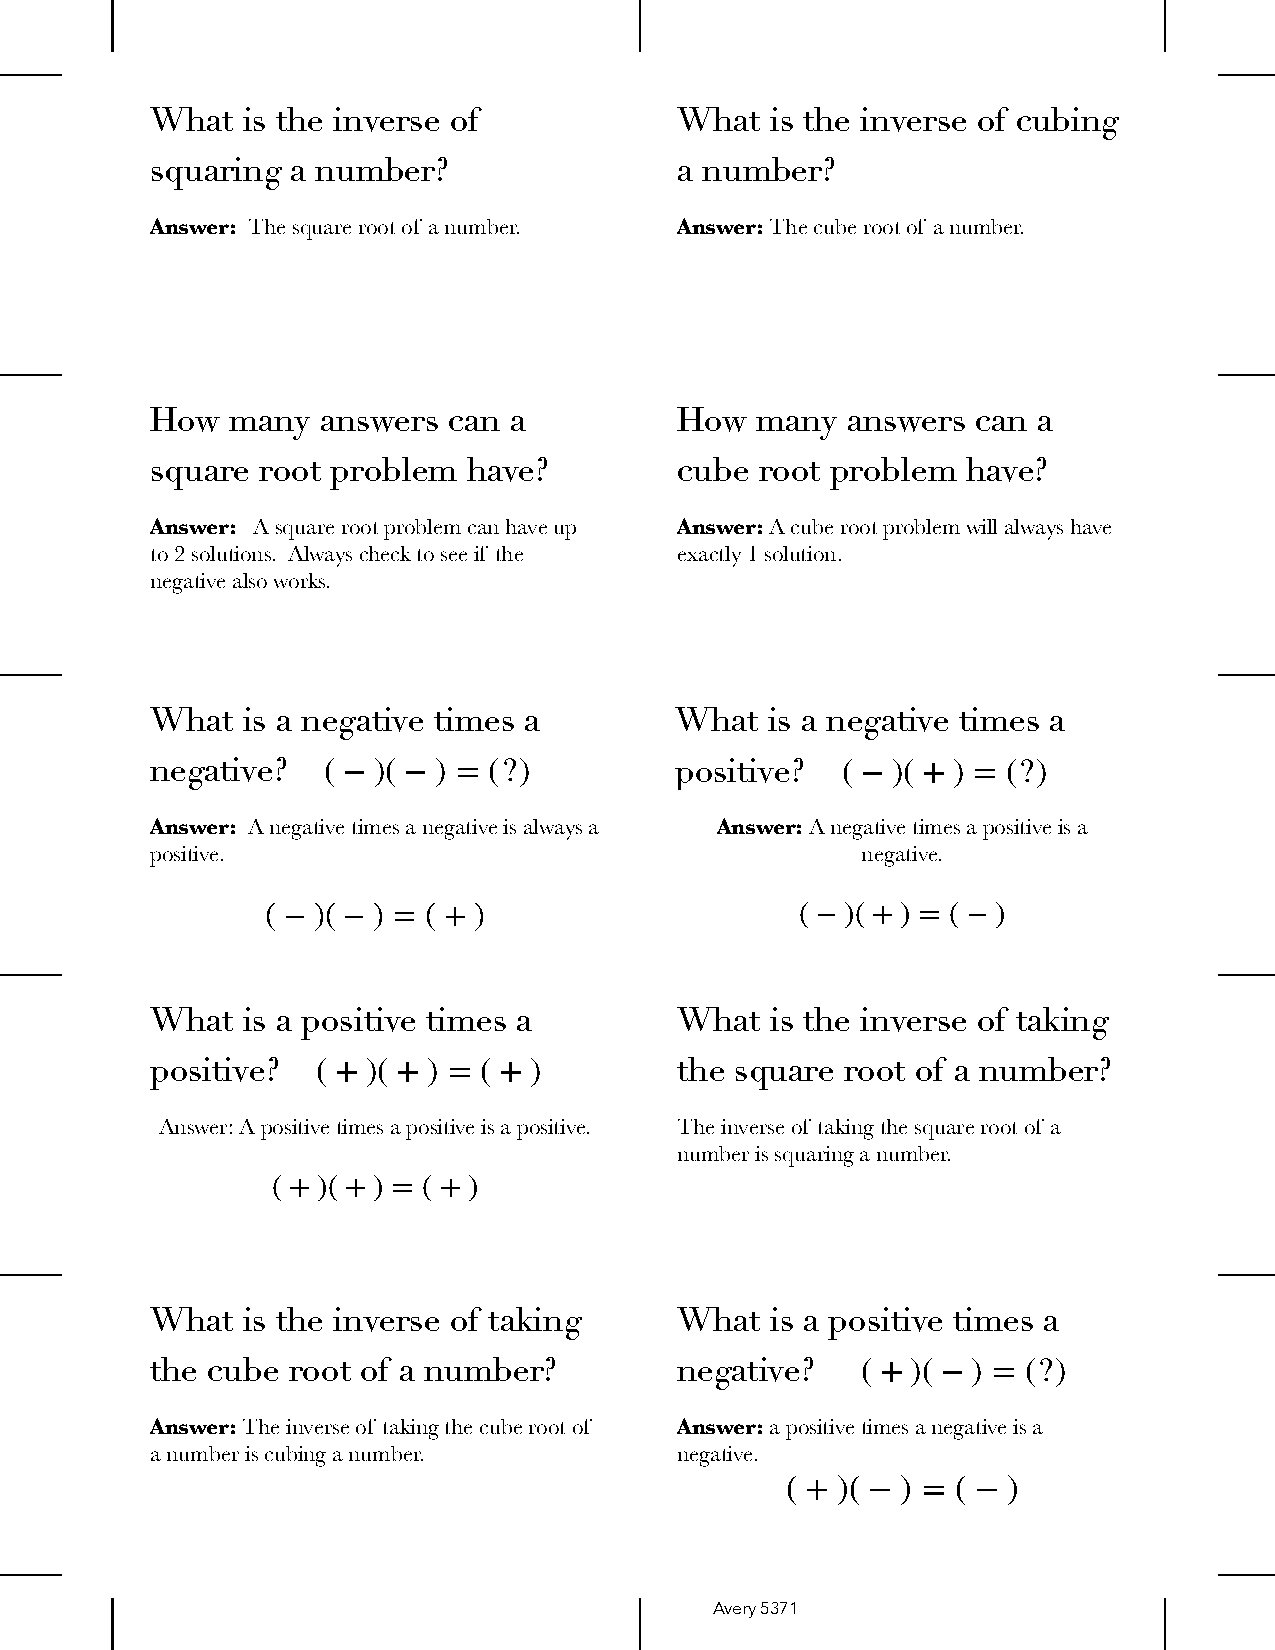
\includepdf[pages=-, scale=0.65]{QQT_square_and_cube.pdf}
    \caption{Quiz-Quiz Trade Cards for practicing vocabulary}
  \end{minipage}
  \label{qqt_root}
\end{figure}

\begin{tabularx}{\textwidth}{Y}
  {\large University of Evansville Lesson Plan Format 8/29/2025} \\
  \arrayrulecolor{blue} \hline \\
\end{tabularx}


\arrayrulecolor{black} 
\begin{tabularx}{\textwidth}{|X|X|}
  \hline 
  \textcolor{blue}{Name:} Randall Helzerman         &   \textcolor{blue}{Student ID Number:} 0128861 \\
  \hline 
  \textcolor{blue}{Course Number:} EDUC-497-03 2025FA &   \textcolor{blue}{Instructor Name:} Dr. Laura Watkins\\
  \hline 
\end{tabularx}
\arrayrulecolor{black}

\vskip 10pt

\begin{tabularx}{\textwidth}{Y}
  {\bf Lesson Overview} \\
\end{tabularx}
\arrayrulecolor{black}


\arrayrulecolor{black} 
\begin{tabularx}{\textwidth}{|X|X|}
  \hline 
  \textbf{Lesson Title:} \\
  
  \hline 
  \textbf{Subject:} Math\\
  
  \hline 
      {
        \begin{tabularx}{\textwidth}{X|X}
          \hskip -6pt
          \textbf{Duration of Lesson: 80 min} & \textbf{Grade Level(s)/Course:} 8th grade\\
        \end{tabularx}
      } \\
      
      \hline
      
      \textbf{Lesson Description: THE PYTHAGOREAN THEOREM} (in all-caps!)\\
      
      \hline
      
      \textbf{Standards and/or Indicator(s):}\\
      \textbf{Indiana Standard number:} 8.GM.8\\
      \textbf{Text:} Apply the Pythagorean Theorem to determine unknown side lengths in right triangles in real-world and other
      mathematical problems in two dimensions.\\
      \hline
      
      \textbf{Learning Objective(s)/Target:} \\
             {\begin{enumerate}
               \item Students should know what a right triangle is
               \item Students should feel comfortable 
             \end{enumerate}} \\
             \hline
             
             \textbf{Lesson Resources/Technology: } 6 3x5 cards for a Pythagorean triple treasure hunt\\
             \hline
             
             \textbf{Key Vocabulary:} 
             Right angle, right triangle, legs of right triangle, hypoteneus of a right triangle. \\
             \hline
\end{tabularx}
\arrayrulecolor{black}

\pagebreak

\begin{tabularx}{\textwidth}{|p{0.5in}|X|}
  \hline
  \centerline{\textbf{\large Time}} &  \textbf{\large Instructional Sequence } \\
  \hline
  \textbf{5 min} &  \textbf{\em Introduction/Anticipatory Set:}     Draw the following figures on the Promethean board: \\
  10 min & 
  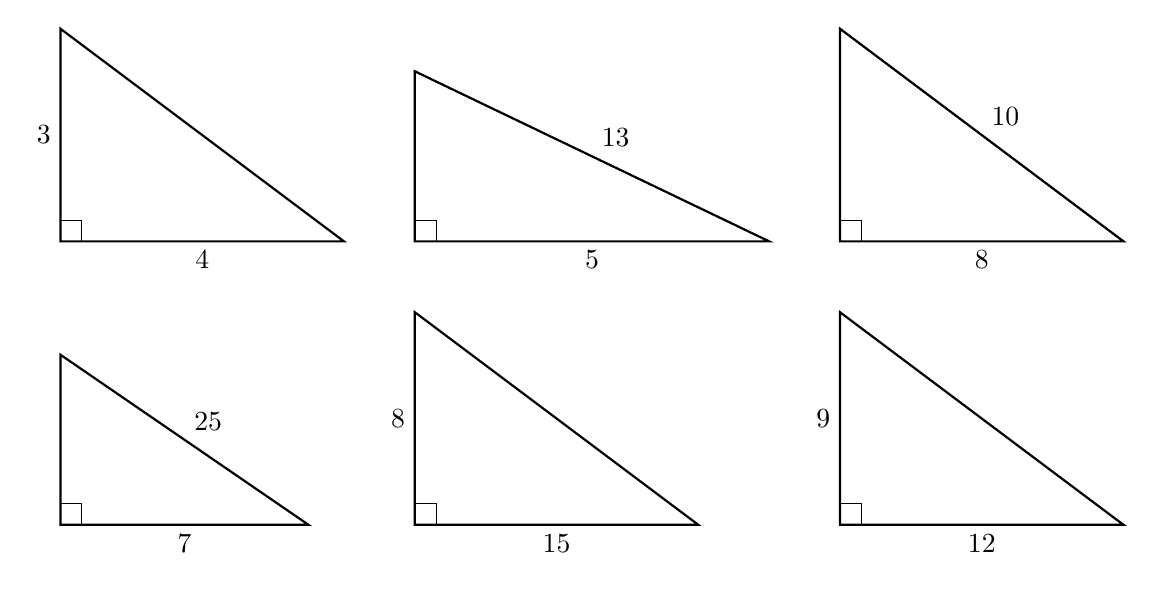
\begin{tikzpicture}[scale=0.9]
    
    % Row 1, Column 1 - Problem 1 (3-4-5 triangle)
    \begin{scope}[shift={(0,0)}]
      \draw[thick] (0,0) -- (4,0) -- (0,3) -- cycle;
      \draw (0.3,0) -- (0.3,0.3) -- (0,0.3);
      \node[below] at (2,0) {4};
      \node[left] at (0,1.5) {3};
    \end{scope}
    
    % Row 1, Column 2 - Problem 2 (5-12-13 triangle)
    \begin{scope}[shift={(5,0)}]
      \draw[thick] (0,0) -- (5,0) -- (0,2.4) -- cycle;
      \draw (0.3,0) -- (0.3,0.3) -- (0,0.3);
      \node[below] at (2.5,0) {5};
      \node[above right] at (2.5,1.2) {13};
    \end{scope}
    
    % Row 1, Column 3 - Problem 3 (6-8-10 triangle)
    \begin{scope}[shift={(11,0)}]
      \draw[thick] (0,0) -- (4,0) -- (0,3) -- cycle;
      \draw (0.3,0) -- (0.3,0.3) -- (0,0.3);
      \node[below] at (2,0) {8};
      \node[above right] at (2,1.5) {10};
    \end{scope}
    
    % Row 2, Column 1 - Problem 4 (7-24-25 triangle)
    \begin{scope}[shift={(0,-4)}]
      \draw[thick] (0,0) -- (3.5,0) -- (0,2.4) -- cycle;
      \draw (0.3,0) -- (0.3,0.3) -- (0,0.3);
      \node[below] at (1.75,0) {7};
      \node[above right] at (1.75,1.2) {25};
    \end{scope}
    
    % Row 2, Column 2 - Problem 5 (8-15-17 triangle)
    \begin{scope}[shift={(5,-4)}]
      \draw[thick] (0,0) -- (4,0) -- (0,3) -- cycle;
      \draw (0.3,0) -- (0.3,0.3) -- (0,0.3);
      \node[below] at (2,0) {15};
      \node[left] at (0,1.5) {8};
    \end{scope}
    
    % Row 2, Column 3 - Problem 6 (9-12-15 triangle)
    \begin{scope}[shift={(11,-4)}]
      \draw[thick] (0,0) -- (4,0) -- (0,3) -- cycle;
      \draw (0.3,0) -- (0.3,0.3) -- (0,0.3);
      \node[below] at (2,0) {12};
      \node[left] at (0,1.5) {9};
    \end{scope}
    
  \end{tikzpicture}  \\

  & Ask the students to write on their whiteboards what the labeled
  sides are for each triangle: Is it the hypoteneus, or a leg? \\
  
  \hline
  
  \textbf{} &

  \textbf{\em Demonstrate, Build, Apply Knowledge} We had a Pythagorean triangle treasure hunt.  At 6 stations around the room there was a problem involving a right triangle, and the solution told the students which station to go to next.  If they arrived back at their first station, they won!  See figure \ref{th_pt} for the cards.\\
  
  \hline
  
  \textbf{} & \textbf{\em Depth of Knowledge Questions:} Had students take out their whiteboards, and list out how many kinds of objects they could see in the room which had right angles.  Let them look around for 5 minutes.

  The students were quite surprised by how many there were.   Some students could name over 50 different kinds of objects (blocks the wall was made of, ceiling tiles, posters on the walls, the walls, etc etc).

  I told them I wanted them to do this exercise because the world they happened to find themselves in is just FULL of right angles, and therefore, right triangles.  And that I wanted them to feel comfortable and safe in their world, and in order to do that, they had to be able to understand their world.   And since their world has so many right angles, a good place to start would be learning the Pythagorean theorem.\\
  
  \hline
  
  \textbf{} & \textbf{\em Guided Practice:} Cold-calling the students, asking them how to identify the variios parts of a right triangle, and how to calculate the lengths of the hypoteneuse.\\
  
  \hline
  
  \textbf{} & \textbf{\em Independent Practice:} Work on some problems from workbook  \\
  
  \hline

  \textbf{} & \textbf{\em Assessment:} We gave an exit ticket to test basic knowledge.\\
  \hline
  
  \textbf{} & \textbf{\em Wrap Up/Closing Activity/Reflection:} N/A\\
  
  \hline
\end{tabularx}
  
\vskip 6pt

\begin{small}
\begin{tabularx}{\linewidth}{|p{2.1in}|X|}
  \hline
  \textbf{Differentiation/Accommodations and/or Modifications: } & Paid more attention to explaining what ``consecutive numbers'' meant.   Most students were not familiar with the word ``consecutive.''\\
  \hline
  \textbf{Culturally Responsive Teaching/ Diversity and Inclusion: } & N/A\\
  \hline
\end{tabularx}

\vskip 6pt

\begin{tabularx}{\linewidth}{|X|}
  \hline
  \textbf{Self-Reflection:} \\
  \textbf{My Teaching:} 
  \begin{enumerate}
  \item After looking at the exit tickets from the first session, it was obvious that I had not done enough explaining what ``consecutive numbers'' were.   I modified my approach and the next session did much better on the exit ticket.
  \item .
  \end{enumerate} \\
  
  \textbf{The Students:}
  \begin{enumerate}
  \item The students really liked the treasure hunt, and they really liked naming out all of the things in the room which had right angles.  
  \item They were amazed that there were so many.  
  \end{enumerate} \\
  
  \textbf{The Lesson:}
  \begin{enumerate}
  \item As noted above, the lesson was a bit thin on explaining what ``consecutive numbers'' were.  
  \end{enumerate} \\
  
  \hline
\end{tabularx}
\end{small}


\begin{figure}[h]
\renewcommand{\arraystretch}{2}
\begin{tabular}{|@{}|c@{\hspace{1cm}}|c@{}|}
  \hline
  & \\
  % Card 1
  \begin{minipage}[t]{3in}
    \centering
    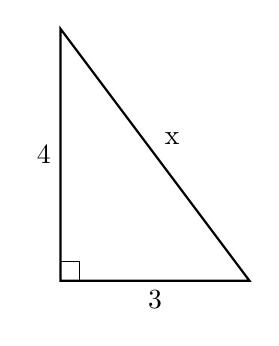
\begin{tikzpicture}[scale=0.8]
      % Triangle
      \draw[thick] (0,0) -- (3,0) -- (0,4) -- cycle;
      % Labels
      \node[below] at (1.5,0) {3};
      \node[left] at (0,2) {4};
      \node[above right] at (1.5,2) {x};
      % Right angle marker
      \draw (0,0.3) -- (0.3,0.3) -- (0.3,0);
    \end{tikzpicture}
    \\[0.5cm]
    Next station: $x-4$
  \end{minipage}
  &
  % Card 2
  \begin{minipage}[t]{3in}
    \centering
    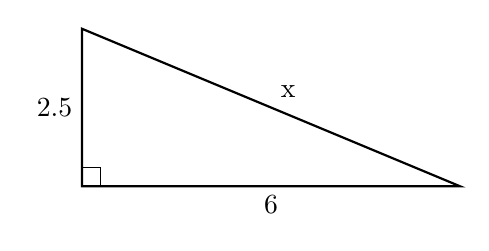
\begin{tikzpicture}[scale=0.8]
      % Triangle
      \draw[thick] (0,0) -- (6,0) -- (0,2.5) -- cycle;
      % Labels
      \node[below] at (3,0) {6};
      \node[left] at (0,1.25) {2.5};
      \node[above right] at (3,1.25) {x};
      % Right angle marker
      \draw (0,0.3) -- (0.3,0.3) -- (0.3,0);
    \end{tikzpicture}
    \\[0.5cm]
    Next station: $x-5$
  \end{minipage}
  \\[1cm]
  \hline
  & \\
  % Card 3
  \begin{minipage}[t]{3in}
    \centering
    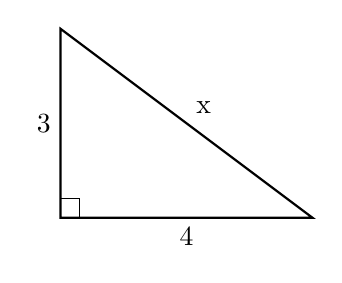
\begin{tikzpicture}[scale=0.8]
      % Triangle
      \draw[thick] (0,0) -- (4,0) -- (0,3) -- cycle;
      % Labels
      \node[below] at (2,0) {4};
      \node[left] at (0,1.5) {3};
      \node[above right] at (2,1.5) {x};
      % Right angle marker
      \draw (0,0.3) -- (0.3,0.3) -- (0.3,0);
    \end{tikzpicture}
    \\[0.5cm]
    Next station: $x-2$
  \end{minipage}
  &
  % Card 4
  \begin{minipage}[t]{3in}
    \centering
    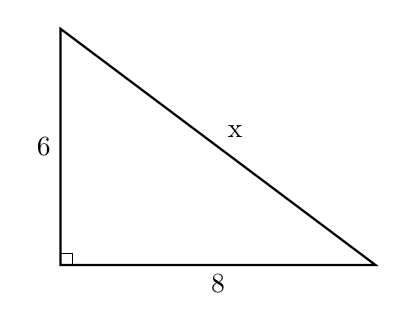
\begin{tikzpicture}[scale=0.5]
      % Triangle
      \draw[thick] (0,0) -- (8,0) -- (0,6) -- cycle;
      % Labels
      \node[below] at (4,0) {8};
      \node[left] at (0,3) {6};
      \node[above right] at (4,3) {x};
      % Right angle marker
      \draw (0,0.3) -- (0.3,0.3) -- (0.3,0);
    \end{tikzpicture}
    \\[0.5cm]
    Next station: $x-4$
  \end{minipage}
  \\[1cm]
  \hline
  & \\
  % Card 5
  \begin{minipage}[t]{3in}
    \centering
    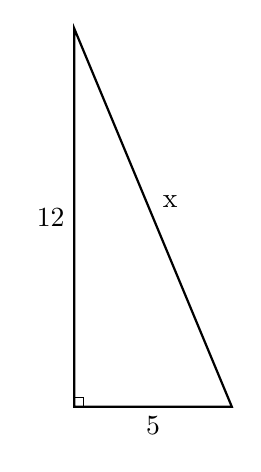
\begin{tikzpicture}[scale=0.4]
      % Triangle
      \draw[thick] (0,0) -- (5,0) -- (0,12) -- cycle;
      % Labels
      \node[below] at (2.5,0) {5};
      \node[left] at (0,6) {12};
      \node[above right] at (2.5,6) {x};
      % Right angle marker
      \draw (0,0.3) -- (0.3,0.3) -- (0.3,0);
    \end{tikzpicture}
    \\[0.5cm]
    Next station: $x-8$
  \end{minipage}
  &
  % Card 6
  \begin{minipage}[t]{3in}
    \centering
    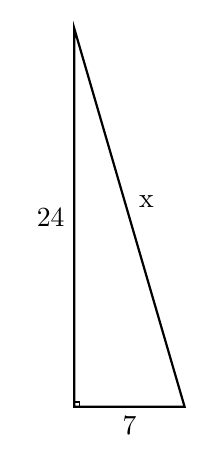
\begin{tikzpicture}[scale=0.2]
      % Triangle
      \draw[thick] (0,0) -- (7,0) -- (0,24) -- cycle;
      % Labels
      \node[below] at (3.5,0) {7};
      \node[left] at (0,12) {24};
      \node[above right] at (3.5,12) {x};
      % Right angle marker
      \draw (0,0.3) -- (0.3,0.3) -- (0.3,0);
    \end{tikzpicture}
    \\[0.5cm]
    Next station: $x-18$
  \end{minipage} \\
  & \\
  \hline
\end{tabular}
\caption{Pythagorean Theorem Practice Problems}
\label{th_pt}
\end{figure}

\chapter{9/2/2025 through 9/9/2025}

\include{lp_sep_2}
\begin{tabularx}{\textwidth}{Y}
  {\large University of Evansville Lesson Plan Format } 9/3/2025 TO 9/4/2025\\
  \arrayrulecolor{blue} \hline \\
\end{tabularx}


\arrayrulecolor{black} 
\begin{tabularx}{\textwidth}{|X|X|}
  \hline 
  \textcolor{blue}{Name:} Randall Helzerman
  &
  \textcolor{blue}{Student ID Number:} 0128861 \\
  \hline
  
  \textcolor{blue}{Course Number:} EDUC-497-03 2025FA
  &
  \textcolor{blue}{Instructor Name:} Dr. Laura Watkins\\
  \hline
  
\end{tabularx}
\arrayrulecolor{black} 

\vskip 10pt
  
\begin{tabularx}{\textwidth}{Y}
  {\bf Lesson Overview} \\
\end{tabularx}
\arrayrulecolor{black}


\arrayrulecolor{black} 
\begin{tabularx}{\textwidth}{|X|X|}
  \hline
  
  \textbf{Lesson Title:} \\
  \hline
  
  \textbf{Subject:} Math\\
  \hline
  
  {\begin{tabularx}{\textwidth}{X|X}
      \hskip -6pt
      \textbf{Duration of Lesson:} & \textbf{Grade Level(s)/Course:}
      8th grade\\
  \end{tabularx}} \\
  \hline
  
  \textbf{Lesson Description: {\tiny (Describe the primary nature
      e.g. hands-on, direct instruction, inquiry, project based
      etc. of the lesson)}} \\
  \hline
  
  \textbf{Standards and/or Indicator(s):} {\tiny Cut and paste from
    IDOE website here. Feel free to replicate the descriptors listed
    below to include more standards in this section.} \\
  
  \textbf{Indiana Standard number:} \\
  
  \textbf{Text:} \\
  
  \hline
  
  \textbf{Learning Objective(s)/Target:} {
    \begin{enumerate}
    \item I can solve simple equations using squares and cubes.
    \item I know how to use the pythagorean theorem to find the length
      of the hypotenuse.
    \end{enumerate}
  }   \\
  \hline
  
  \textbf{Lesson Resources/Technology: } Promethean board \\
  \hline
  
  \textbf{Key Vocabulary:} \\ square, square root, cube, cube root,
  consecutive, hypotenuse, pythagorean theorem, operator, inverse
  operator. \\
  \hline
  
\end{tabularx}
\arrayrulecolor{black}

\pagebreak

\begin{tabularx}{\textwidth}{|p{0.5in}|X|}
  \hline
  
  \centerline{\textbf{\large Time}} &  \textbf{\large Instructional Sequence } \\
  
  \hline
  
  \textbf{} & \textbf{\em Introduction/Anticipatory Set:} Write the following simple equtions on the whiteboard:
  \[
    \begin{array}{c c c}
      c^{2}=15  & c^{2}=35  & c^{2}=8 \\
      c^{2}=27  & c^{2}=12  & c^{2}=17 \\
    \end{array} \]

   and ask the students to solve.  Then go over their answers. \\
  \hline
  
  \textbf{} & \textbf{\em Demonstrate, Build, Apply Knowledge}  N/A\\
  \hline
  
  \textbf{} & \textbf{\em Depth of Knowledge Questions:} N/A \\
  \hline
  
  \textbf{} & \textbf{\em Guided Practice:}   Worked a few problems on the study guide on the board.\\
  \hline
  
  \textbf{} & \textbf{\em Independent Practice:}  Study guide for test tomorrow. \\
  \hline
  
  \textbf{} & \textbf{\em Assessment:}  Test tomorrow \\
  \hline
  
  \textbf{} & \textbf{\em Wrap Up/Closing Activity/Reflection:} N/A \\
  \hline 
\end{tabularx}

\vskip 6pt

\begin{small}
  \begin{tabularx}{\linewidth}{|p{2.1in}|X|}
    \hline
    \textbf{Differentiation/Accommodations and/or Modifications: } & N/A\\
    \hline
    \textbf{Culturally Responsive Teaching/ Diversity and Inclusion: } & N/A\\
    \hline
  \end{tabularx}
  
  \vskip 6pt

  \begin{tabularx}{\linewidth}{|X|}
    \hline
    \textbf{Self-Reflection:} \\
    \textbf{My Teaching:} 
    \begin{enumerate}
    \item Made a critical mistake: emphasized that we want the answer to
      be consecutive whole numbers, but then explained how to solve the
      problems by advertint to perfect squares, which are not
      consecutive.  This confused a lot of students.  Fortunatey I fixed
      in in the subsequent presentations.
    \end{enumerate} \\
    
    \textbf{The Students:}
    \begin{enumerate}
    \item The students have a rather limited vocabulary, and we have to
      be sensitive to that.  The word ``consecutive'' was new to them,
      and it took a few days for them to wrap their heads around it.
    \end{enumerate} \\
2    
    \textbf{The Lesson:}
           \begin{enumerate}
             \item We are trying to adhere to the prescribed lessons as much as
               possible, but this particular unit did not seem to have very
               effective structure.  To the students, it just seem like a grab-bag of ad-hoc techniques.
             \item They are not in algebra class, but yet we are teaching them
               bits and pieces of algebra in order for them to be able to solve
               the problems.   It seems like presenting the rules for, say, canceling a square root with a square, would be easier to understand as part of a larger system of canceling addition with subtraction, etc.  
           \end{enumerate} \\
           
           \hline
\end{tabularx}
\end{small}


\section{Spotlight on Student ``S''}

Student S reminds me of the character of Bartlby in Herman Melville's
short story ``Bartlby the Scriviner.''  In class he is unfailingly
polite, and never disrupts class in any way.  In fact, it appears that
he has absolutely no motivation to do anything, and is just passing
his time.  In class, he is completely passive.  He zones out as soon
as the teacher starts speaking and pays absolutly no attention.  If
prompted to take notes, he politey declines, and resumes his silence.

Ordinarily, I would suspect that he is somewhere on the autistic
spectrum, but in this case, his sphinx-like appearances are decieving.
He was professionally evauated, and is not autistic at all.  Indeed,
he is only passive and silent in class.  At lunchtime and at recess
with his friends, he is as animated and conversational as any other
student.  But when he comes back to class, he once again renews his
vow of silence, and nothing can disturb his zen.

S is in the 8th grade, and apparently, the faculty have been actively
trying to engage him since he entered middle school in the 6th grade.
These efforts have not entirely been in vain.  At the beginning of the
year, he actually answered a question in the community circle!
Mrs. Toelle about fainted to hear him speak.  The question was ``what
is your favorite thing to do?'' and he answered ``baking pastries.''
He even answered a followup question about what his favorite pastry to bake was,
answering ``Tiramasu.''

As hugh as these gains are in relative terms, in absolute terms,
student S is very far from where he needs to be.  This week, there was
an all-hands faculty meeting about him.  They are very worried that if
he maintains his anchoratage through high school, he will have
sucessfully managed to entirely defend himself against getting an
education.

In one of the exercises in the faculty meeting, the Vice Principal
asked us to think about what kind of intervention might be effective
for student S.  She had a slide of many different possibilities on the
screen, and one caught my eye.  It caught my eye because I had used
the technique on {\em myself} at times when I felt solidarity with
Bartlby and with student S, in prefering rather not to do my homework,
or read a paper I needed to.

The technique is the one used in the so-called ``Pomodoro'' method:
Instead of viewing the task as a huge, long task which mentaly
exhausts you just thinking about it, resolve instead to work on it for
a limited time.  For me, a time which worked was 5 minuges.  I can
endure anything for 5 minutes.  For Student S, I thought that perhaps
20 seconds would be a more apropos time.

I got my chance to try it out when student S was pulled for small group
which I tutored.  I pulled out my watch, and said that he only had to
pay attention to my explanation for 20 seconds, and then I'd let him
rest.  I quickly explained how to work a problem, and let him rest for
30 seconds while I checked up on the other students in the small
group.  Then, I told him ``you only have to work these example
problems for 20 seconds, then you can rest again.''  He wanted to
decline, but I said, ``hey, the misery will be over in 20 seconds,
then you can rest again.''  So he tried, and actually did 2 problems in
the 20 seconds.   Amazing.

I went through about 3 more rounds of this before the allotted time
with the small group expired, and student S was quite ready to quit.
He had put his head down on the table.

But this time, it wasn't because he was just politely declining--I
think he was genuinely mentally exhausted, inasmuch as this might have
been as much sustaied schoolwork he has done in a decade.

So a glimmer of hope at least.  Several obstacles are in the way of
tryhing this out on a larger scale:
\begin{enumerate}
\item it was hard to do what was in effect two lessons simultaneously--one for student S, and the other for the other students in the small group.  I had to continuously interrupt myself to go tend to student S.
\item I have no training in how far to push him.  After 3 rounds he looked very tired to me, but if I had the time, could I have pushed him further?  How far is too far?
\item Obviously, the time he's concentrating has to go from 20 seconds to a more normal 5-10 minutes like the rest of his generation's unfortunately vestigial attention span is.  How fast can this be done?
\end{enumerate}
\noindent At any rate, on Monday I'll have a chat with Mrs. Toelle and the Vice Principal.  Hopefully we'll be able to get through to him.


\end{document}
